\chapter{State of the Art}
\label{chap:sota}  

\section*{Introduction}
This chapter provides a comprehensive review of the state-of-the-art in cooperative multi-agent reinforcement learning, with a specific focus on methods designed to address the challenge of partial observability. We begin by analyzing the foundational algorithms within the CTDE paradigm, such as Value-Decomposition Networks (VDN) and QMIX, which form the bedrock of modern cooperative MARL. We then transition to more advanced representation learning techniques that explicitly tackle the problem of missing information. This thematic analysis covers belief alignment methods like COLA, contrastive learning frameworks such as MA2CL, and, most critically, the reconstruction-based approach of the Multi-Agent Masked Auto-Encoder (${MA}^2E$), which serves as the direct foundation for our work. By critically evaluating the strengths and limitations of these approaches, this chapter establishes the research gap for a more adaptive and efficient masking strategy.

\section{Key Concepts and Terminology}

Before delving into the specific algorithms, this section defines several key concepts and recurring terminologies that are central to the state-of-the-art in cooperative MARL, particularly those addressing partial observability.

\paragraph{Value Decomposition}
A dominant strategy in value-based CTDE algorithms where the goal is to learn the global, joint action-value function ($Q_{tot}$) by factorizing it into individual utility functions ($Q_i$), one for each agent[cite: 2320, 736]. Foundational methods like VDN assume a simple summation, while more advanced methods like QMIX use a non-linear mixing network to combine the individual utilities.

\paragraph{The Monotonicity Constraint (IGM Principle)}
A crucial innovation introduced in QMIX that constrains its mixing network, ensuring that an increase in any individual agent's utility, $Q_i$, cannot cause a decrease in the total team value, $Q_{tot}$.This property is a sufficient condition to guarantee the Individual-Global-Max (IGM) principle, which ensures that a greedy action selection by each decentralized agent corresponds to the maximization of the global value function, making it critical for effective decentralized execution.

\paragraph{Centralized Critic}
A core component of policy-gradient-based CTDE methods like MADDPG and MAPPO.The critic is a value function that is used only during the training phase and is given access to global information, such as the full state and the actions of all agents. This allows it to provide a stable, low-variance learning signal (i.e., policy gradient) to guide the training of the decentralized actors (the agents' individual policies).

\paragraph{Advanced Representation Learning}
This refers to a class of techniques that aim to overcome the limitations of using a standard RNN to handle partial observability. Instead of just compressing an agent's history into a memory state, these methods focus on explicitly learning richer features or representations from partial observations. The goal is to allow agents to directly reason about or infer missing information about the true global state, either by aligning beliefs (like COLA) or by reconstructing the missing information (like ${MA}^2E$).

\paragraph{Masked Modeling}
A self-supervised learning paradigm where a model learns to reconstruct original data from a corrupted input, where parts have been "masked" or removed. This approach, popularized in NLP and computer vision, forces the model to learn a deep, contextual understanding of the data's underlying structure. In the context of MARL, this involves masking the trajectories of some agents and training a model to reconstruct them, thereby learning to infer global information from a partial view.
\section{Thematic Analysis}
% \lipsum[2]
% \subsection{Motivating Application: Coordination of  Unmanned Aerial Vehicles (UAVs) }
% A primary obstacle in applying reinforcement learning to robotics is the \textit{sim-to-real gap}: the significant discrepancy between the idealized physics and clean data of a simulator and the noisy, unpredictable dynamics of the physical world. A policy trained exclusively in a perfect simulation will likely fail upon deployment because it has not learned to handle real-world complexities like sensor noise, actuator lag, or environmental variations like wind. To address this critical challenge,\parencite{adversarial_domain_randomization} proposes a robust MARL framework designed to create policies that successfully transfer from simulation to real UAVs.

% Their approach is centered on a sophisticated technique known as \textbf{adversarial domain randomization (ADR)}. To understand ADR, it is useful to first consider standard domain randomization, where parameters of the simulation (e.g., mass, friction, lighting) are randomly varied during training. This exposes the agent to a range of conditions, preventing it from overfitting to a single, perfect simulation model. ADR enhances this process by introducing a second machine learning agent \textbf{an adversary} whose goal is to actively find the most difficult set of environmental parameters to make the primary agents fail. This creates an intelligent and adaptive training curriculum. Instead of randomly encountering challenging scenarios, the adversary systematically generates worst-case conditions, forcing the main agents to learn policies that are maximally robust.

% This adversarial training is complemented by an improved experience replay mechanism that prioritizes transitions with high temporal difference (TD) errors. This focuses the learning process on the most surprising or informative events, enhancing both training stability and sample efficiency.

% \paragraph{Strength} The key contribution of this work is a powerful method for bridging the sim-to-real gap, producing highly robust policies that generalize well from simulation to tangible, real-world UAV deployment.

% \paragraph{Limitations} However, the framework's focus is squarely on the sim-to-real problem for individual agent robustness. It does not fundamentally address the core MARL challenge of partial observability that arises from inter-agent interactions, nor is it designed to scale to large, complex swarms where decentralized coordination is the primary bottleneck.
%--------- old ---------------------------------------------------
% While some research focuses on the sim-to-real problem, \parencite{fuzzy_maddpg} tackles the challenge of coordination in uncertain, communication-limited environments, such as multi-UAV search and rescue. They propose a Fuzzy Deep Reinforcement Learning (Fuzzy-DRL) framework that enhances the popular MADDPG algorithm by integrating two key concepts: fuzzy logic and entropy-based rewards.

% Fuzzy logic is a powerful mathematical framework for reasoning with imprecise or incomplete information.
% %, moving beyond the traditional binary logic of ``true'' or ``false.'' Instead of requiring precise numerical inputs (e.g., ``distance is exactly 20.5 meters''), it allows for reasoning with linguistic variables that have degrees of truth (e.g., a UAV can be considered ``close,'' ``nearby,'' or ``far''). 
% In this context, fuzzy rules are used to intelligently manage the agents' reliance on communication. 
% % For example, a rule might state: ``IF an ally is 'very close' AND my task uncertainty is 'low', THEN my reliance on their communicated message is 'very low'.''
% This allows the system to gracefully handle intermittent or noisy communication without catastrophic failure.

% To improve the agents' ability to explore their environment, the authors incorporate entropy-based rewards. In reinforcement learning, entropy is a measure of the randomness or unpredictability of an agent's policy. By adding the entropy of its action distribution to the main task reward, the agent is intrinsically rewarded for trying new and diverse actions, preventing it from prematurely converging to a suboptimal strategy.

% \paragraph{Strength} The primary advantage of this hybrid method is its ability to create robust coordination strategies that can better handle the uncertainty inherent in real-world environments, particularly when communication is unreliable or limited.

% \paragraph{Limitation} The framework's main drawback lies in its scalability. Fuzzy logic systems rely on a set of human-engineered rules. As the number of agents and the complexity of their interactions increase, designing, managing, and tuning this rule set can become complex, making the approach less scalable than methods that learn all behaviors end-to-end.
%--------- old ---------------------------------------------------

% While some research focuses on the \textbf{sim-to-real} problem, \parencite{fuzzy_maddpg} tackles the challenge of coordination in uncertain, communication-limited environments typical of multi-UAV search and rescue. They propose a \textbf{Fuzzy Deep Reinforcement Learning (Fuzzy-DRL)} framework that enhances the popular \textbf{MADDPG} algorithm by integrating two key concepts: \textbf{fuzzy logic} and \textbf{entropy-based} rewards.

% The first component, fuzzy logic, is introduced to handle ambiguity and reason with imprecise data. Unlike classical logic, which operates on binary true/false values, fuzzy logic uses degrees of truth, allowing variables to belong partially to different sets. It operates on linguistic variables (e.g., distance can be described as \textit{close} or \textit{far}) which are mapped via membership functions to a value between 0 and 1. In this framework, fuzzy rules intelligently modulate the weight given to communicated information from teammates based on factors like distance or data uncertainty. This mechanism allows the system to gracefully degrade its reliance on communication when it is noisy or unavailable, preventing catastrophic failures and enhancing operational robustness.

% To improve the agents' learning process, the authors incorporate \textbf{entropy-based rewards}. In information theory, entropy quantifies the uncertainty or randomness in a distribution. Within reinforcement learning, adding an entropy bonus to the reward function drives the agent to maintain a more stochastic policy (one that does not collapse to a single, deterministic action for a given state ). This has two benefits: it drives better exploration during training by encouraging the agent to try diverse actions, and it results in a less predictable final policy, which can be more robust in complex, dynamic environments.

% The primary strength of this hybrid method is its ability to produce coordination strategies that are inherently more resilient to environmental uncertainty and unreliable communication. However, the framework's main drawback is its scalability. Fuzzy logic systems depend on a set of human-engineered rules and membership functions. As the number of agents and the complexity of their interactions grow, the design and tuning of this rule-based system can become combinatorially complex, making the approach difficult to scale compared to end-to-end learning methods.
% To more directly address the core challenge of partial observability in multi-agent systems,\parencite{collaborative_decision-making} introduces a MARL method for multi-UAV collaboration built on a sophisticated actor-critic architecture. Their framework's novelty lies in the explicit combination of two powerful neural network components: recurrent networks and attention mechanisms.

% First, to handle the temporal nature of partial observability, each agent's policy is equipped with a Recurrent Network (RNN), such as a Gated Recurrent Unit (GRU) or Long Short-Term Memory (LSTM). An RNN processes sequences of observations, maintaining an internal hidden state that acts as a memory. This allows the agent to build a \textit{belief} or context from its observation history, rather than reacting solely to its most recent perception, which is crucial in environments where the full state is not visible at once.

% Building on this memory-based approach, the authors integrate an attention mechanism. While an RNN provides a compressed history, not all past information is equally relevant to the current decision. The attention mechanism allows the model to dynamically weigh the importance of different parts of its input, be it different elements of its own observation history or information communicated by different teammates. By learning to focus on the most salient information, the agent can make more informed and contextually aware decisions.

% The primary strength of this combined architecture is its ability to significantly improve coordination in partially observable settings by equipping agents with both a robust memory (from RNNs) and a method for selective focus (from attention). However, this enhanced capability comes with a significant limitation: both recurrent and attention layers add considerable computational complexity. This results in a model that is more computationally expensive and parameter-heavy, leading to longer training times and reduced efficiency, which can hinder its application in large-scale systems.
% \subsection{Motivating Application: Coordination of Unmanned Aerial Vehicles (UAVs)}
\subsection{Coordination of Unmanned Aerial Vehicles (UAVs)}
Research in multi-agent UAV coordination has produced solutions for several distinct challenges. To bridge the critical \textit{sim-to-real gap}, where policies trained in simulators fail in the real world, \parencite{adversarial_domain_randomization} uses adversarial domain randomization. This technique employs an adversary to generate worst-case environmental conditions in the simulator, forcing the agents to learn highly robust policies. While powerful for sim-to-real transfer, this method does not fundamentally address the MARL challenge of partial observability.

% To handle coordination under communication uncertainty, \parencite{fuzzy_maddpg} enhance the \textbf{MADDPG} algorithm with a \textit{Fuzzy-DRL} framework. This method uses pre-defined fuzzy logic rules to intelligently manage unreliable communication and incorporates \textit{entropy-based rewards}  to encourage exploration. The resulting system is more resilient to communication loss, but its reliance on hand-crafted fuzzy rules creates a significant scalability bottleneck.

To handle coordination under communication uncertainty, \parencite{fuzzy_maddpg} enhances the \textbf{MADDPG} algorithm with a \textit{Fuzzy Deep Reinforcement Learning} (Fuzzy-DRL) framework. This approach integrates two key concepts: \textit{fuzzy logic} and \textit{entropy-based rewards}. The first component, fuzzy logic, is introduced to manage ambiguity by reasoning with linguistic variables (e.g., describing distance as \textit{close} or \textit{far}) rather than relying on precise numerical values. Within this framework, human-engineered fuzzy rules intelligently modulate the weight assigned to information communicated by teammates based on factors such as distance or data uncertainty. This enables the system to gracefully handle noisy or intermittent communication, thereby enhancing operational robustness. To further improve learning, the authors incorporate entropy-based rewards: by adding an entropy bonus to the reward function, the agent is implicitly encouraged to maintain a more stochastic policy, which improves exploration and results in a more robust and less predictable final policy. While the system is highly tolerant of communication loss, its reliance on a hand-crafted rule set introduces a significant scalability limitation as the number of agents and the complexity of their interactions increase.

More directly addressing partial observability,
\parencite{collaborative_decision-making} combine Recurrent Networks (RNNs) to provide agents with a memory of past observations, and attention mechanisms to allow them to focus on the most salient information within that memory. This combination of memory and selective focus improves coordination, but at the cost of significant computational complexity that hinders its use in large-scale systems.

Collectively, these approaches highlight that targeted solutions for specific UAV problems often introduce scalability challenges or do not solve the underlying representation problem of partial observability, motivating the need for more general and efficient methods discussed next.
\subsection{The CTDE Paradigm and its Core Implementations}
\label{subsec:ctde}
Research within the CTDE paradigm has produced several algorithmic families designed to balance effective learning with scalable execution. These methods learn centrally but act decentrally, and are broadly categorized into value-decomposition and policy-gradient approaches.

% \paragraph{Value-Decomposition Network (VDN)}
% The foundational value-decomposition method is the Value-Decomposition Network (VDN), introduced by \parencite{VDN}. Its core mechanic is to learn a decomposed representation of the team's joint action-value function, $Q_{\text{tot}}$, by assuming it can be represented as a simple sum of individual agents' utility functions, $Q_i$, each conditioned only on an agent's local observation-action history. The total team value is thus calculated according to Equation~\eqref{eq:vdn}:

% \begin{equation}
%     \label{eq:vdn}
%     Q_{\text{tot}}(\tau,u) = \sum_{i=1}^{n} Q_i(\tau_i, u_i)
% \end{equation}

% where:
% \begin{itemize}
%     \item $Q_{\text{tot}}(\tau, u)$ is the total action-value for the team, given the joint action-observation history $\tau$ and the joint action $u$.
%     \item $Q_i(\tau_i, u_i)$ is the individual utility function learned by agent $i$, based on its own local history $\tau_i$ and its individual action $u_i$.
%     \item $n$ is the total number of agents.
% \end{itemize}

% During training, VDN uses a shared replay buffer to calculate the TD-error based on this global $Q_{\text{tot}}$, and the resulting loss is backpropagated through the summation to implicitly update each individual $Q_i$ network without needing agent-specific rewards. The primary advantage of this structure is that it enables efficient, decentralized execution; since maximizing the sum of the utilities is equivalent to maximizing each one individually, each agent can simply act greedily with respect to its own local utility function during deployment. This makes the approach highly scalable and more effective than fully centralized or independent learning methods. However, VDN's fundamental drawback lies in its restrictive additive assumption. By forcing a linear decomposition, VDN cannot represent more complex, non-linear interactions between agents where one's contribution is conditional on the actions of others.
% \begin{figure}
%     \centering
%     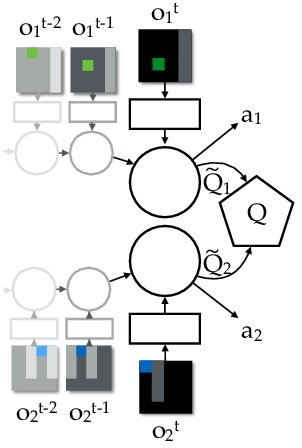
\includegraphics[width=0.5\linewidth]{img_pfe/vdn.png}
%     \caption{Enter Caption}
%     \label{fig:vdn}
% \end{figure}
The foundational value-decomposition method is the Value-Decomposition Network (VDN), introduced by \parencite{VDN}. Its core mechanic is to learn a decomposed representation of the team's joint action-value function, $Q_{\text{tot}}$, by assuming it can be represented as a simple sum of individual agents' utility functions, $Q_i$. The VDN architecture, illustrated for a two-agent case in Figure~\ref{fig:vdn_architecture}, shows how each agent's network processes its own local observation history ($\tau_i$) to produce an individual utility value ($\tilde{Q}_i$). These individual values are then combined by a simple summation to produce the total team value, $Q_{\text{tot}}$. The total team value is thus formally calculated as shown in Equation~\eqref{eq:vdn}:



\begin{equation}
    \label{eq:vdn}
    Q_{\text{tot}}(\tau,u) = \sum_{i=1}^{n} Q_i(\tau_i, u_i)
\end{equation}

Where:
\begin{itemize}
    \item $Q_{\text{tot}}(\tau, u)$ is the total action-value for the team, given the joint action-observation history $\tau$ and the joint action $u$.
    \item $Q_i(\tau_i, u_i)$ is the individual utility function learned by agent $i$, based on its own local history $\tau_i$ and its individual action $u_i$.
    \item $n$ is the total number of agents.
\end{itemize}

During training, VDN uses a shared replay buffer to calculate the TD-error based on this global $Q_{\text{tot}}$, and the resulting loss is backpropagated through the summation to implicitly update each individual $Q_i$ network without needing agent-specific rewards. The primary advantage of this structure is that it enables efficient, decentralized execution; since maximizing the sum of the utilities is equivalent to maximizing each one individually, each agent can simply act greedily with respect to its own local utility function during deployment. This makes the approach highly scalable and more effective than fully centralized or independent learning methods. However, VDN's fundamental drawback lies in its restrictive additive assumption. By forcing a linear decomposition, VDN cannot represent more complex, non-linear interactions between agents where one's contribution is conditional on the actions of others.
% \begin{figure}[H] 
%     \centering
%     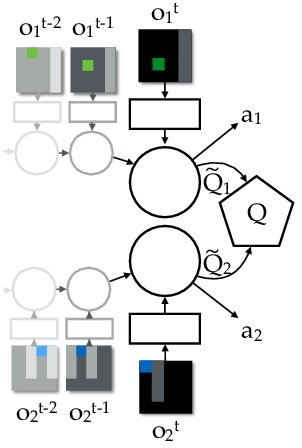
\includegraphics[width=0.3\textwidth]{img_pfe/vdn.png} 
%     \caption{The architecture of a Value-Decomposition Network (VDN) for two agents. Each agent's network processes local observations ($O_1, O_2$) through recurrent layers to produce individual utility values ($\tilde{Q}_1, \tilde{Q}_2$). These are then summed to form the joint Q-value ($Q$), which is used for centralized training. (Adapted from \parencite{VDN}).}
%     \label{fig:vdn_architecture}
% \end{figure}
% Use the standard 'figure' environment as a floating wrapper
% This is the code for your side-caption figure.
% It uses minipage and is fully compatible with the 'caption' package.

\begin{figure}[H]
    
    % --- Box for the image ---
    % I've set its width to 35% of the text width.
    \begin{minipage}{0.3\textwidth}
        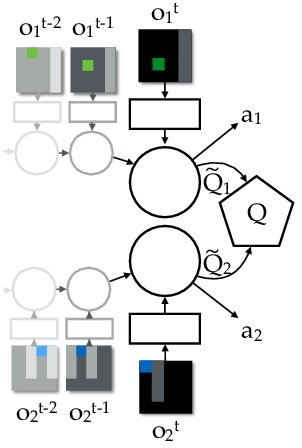
\includegraphics[width=\linewidth]{img_pfe/vdn.png}
    \end{minipage}
    \hspace{0.07\textwidth} 
    \begin{minipage}{0.5\textwidth}

        \captionof{figure}{The architecture of a Value-Decomposition Network (VDN) for two agents. Each agent's network processes local observations ($O_1, O_2$) through recurrent layers to produce individual utility values ($\tilde{Q}_1, \tilde{Q}_2$). These are then summed to form the joint Q-value ($Q$), which is used for centralized training. (Adapted from \parencite{VDN}).}
        \label{fig:vdn_architecture}
    \end{minipage}

\end{figure}
% \paragraph{QMIX}
% To address the expressive limitations of VDN, QMIX was introduced as a more sophisticated value-decomposition algorithm. QMIX replaces the simple summation with a non-linear mixing network that takes all individual agent utilities, $Q_i$, as input to produce the team value, $Q_{\text{tot}}$. The crucial innovation is that the weights of this mixing network are constrained to be non-negative, enforcing an overall monotonicity constraint on the relationship between individual and team values:
% $$
% \frac{\partial Q_{\text{tot}}}{\partial Q_i} \geq 0
% $$
% This elegant constraint guarantees the Individual-Global-Max (IGM) principle, which ensures that a greedy action selection by each decentralized agent still leads to the maximization of the global team value. This allows QMIX to represent a much richer class of functions than VDN, capturing more complex agent synergies while still permitting tractable decentralized execution. Despite its advantages, the monotonicity requirement still imposes a structural constraint on the types of value functions that can be learned, which may not be sufficient for all possible multi-agent coordination problems.
% To address the expressive limitations of VDN, QMIX, introduced by \parencite{QMIX}, provides a more sophisticated value-decomposition approach. QMIX replaces the simple summation with a non-linear mixing network that takes all individual agent utilities, $Q_i$, as input to produce the team value, $Q_{\text{tot}}$. The overall architecture, depicted in Figure~\ref{fig:qmix_architecture}, consists of individual agent networks (c) that produce utility values, which are then fed into a central mixing network (b). The crucial innovation of QMIX lies in this mixing network (a), which enforces a monotonicity constraint on the relationship between individual and team values:
% \begin{equation*}
%     \frac{\partial Q_{\text{tot}}}{\partial Q_i} \geq 0
% \end{equation*}
% This is achieved by using hypernetworks (in red) that take the global state $s_t$ as input and generate the weights for the mixing network, ensuring they are non-negative. The entire end-to-end system is then trained to minimize a standard temporal-difference loss over the joint action-value function, as shown in Equation~\eqref{eq:qmix_loss}:



% \begin{equation}
%     \label{eq:qmix_loss}
%     L(\theta) = \sum_{i=1}^{b} \left[ \left(y^{i}_{\text{tot}} - Q_{\text{tot}}(\tau, u, s; \theta)\right)^2 \right]
% \end{equation}

% where:
% \begin{itemize}
%     \item $L(\theta)$ is the loss function parameterized by the network weights $\theta$.
%     \item $b$ is the batch size of transitions sampled from the replay buffer.
%     \item $Q_{\text{tot}}(\tau, u, s; \theta)$ is the joint action-value function produced by the mixing network.
%     \item $y_{\text{tot}}$ is the target value (TD target), calculated as: 
%     \begin{equation*}
%          y_{\text{tot}} = r + \gamma \max_{u'} Q_{\text{tot}}(\tau', u', s'; \theta^{-})
%     \end{equation*}
   
%     where $\theta^{-}$ represents the parameters of a periodically updated target network.
% \end{itemize}

To address the expressive limitations of VDN, QMIX, introduced by  \parencite{QMIX}, provides a more sophisticated value-decomposition approach. It replaces the simple summation with a non-linear mixing network that takes all individual agent utilities, $Q_i$, as input to produce the team value, $Q_{\text{tot}}$. The overall architecture, depicted in Figure~\ref{fig:qmix_architecture}, shows how individual agent networks feed their utilities into this central mixing network. The crucial innovation of QMIX lies in enforcing a monotonicity constraint on this network, ensuring that an increase in any individual utility does not cause a decrease in the team value:
\begin{equation*}
    \frac{\partial Q_{\text{tot}}}{\partial Q_i} \geq 0
\end{equation*}
This is achieved by using hypernetworks that take the global state $s_t$ as input and generate non-negative weights for the mixing network, allowing the system to leverage centralized information during training.

The entire end-to-end system is trained by minimizing a temporal-difference (TD) loss function over batches of experience sampled from a replay buffer. This loss is defined as:
\begin{equation}
    \label{eq:qmix_loss}
    L(\theta) = \sum_{i=1}^{b} \left[ \left(y_{\text{tot}} - Q_{\text{tot}}(\tau, u, s; \theta)\right)^2 \right]
\end{equation}
Here, the target value $y_{\text{tot}}$ is calculated using the standard Bellman update,\begin{equation*}
    y_{\text{tot}} = r + \gamma \max_{u'} Q_{\text{tot}}(\tau', u', s'; \theta^{-})
\end{equation*}
, where $r$ is the team reward, $\gamma$ is the discount factor, and $\theta^{-}$ are the parameters of a separate, periodically updated target network.

The primary advantage of this monotonic design is that it is a sufficient condition to guarantee the \textbf{Individual-Global-Max (IGM) } principle. The IGM principle ensures that a greedy action selection by each decentralized agent still corresponds to the maximization of the global team value, which is critical for effective decentralized execution. This allows QMIX to represent a much richer class of non-linear functions than VDN while maintaining tractability. However, despite its advantages, the monotonicity constraint also forms the primary limitation of QMIX, as it cannot represent non-monotonic value functions that can arise in problems where an agent's best action depends on the simultaneous actions of its teammates.
\begin{figure}[H]
    % \centering
    \begin{minipage}{0.6\textwidth}
        
    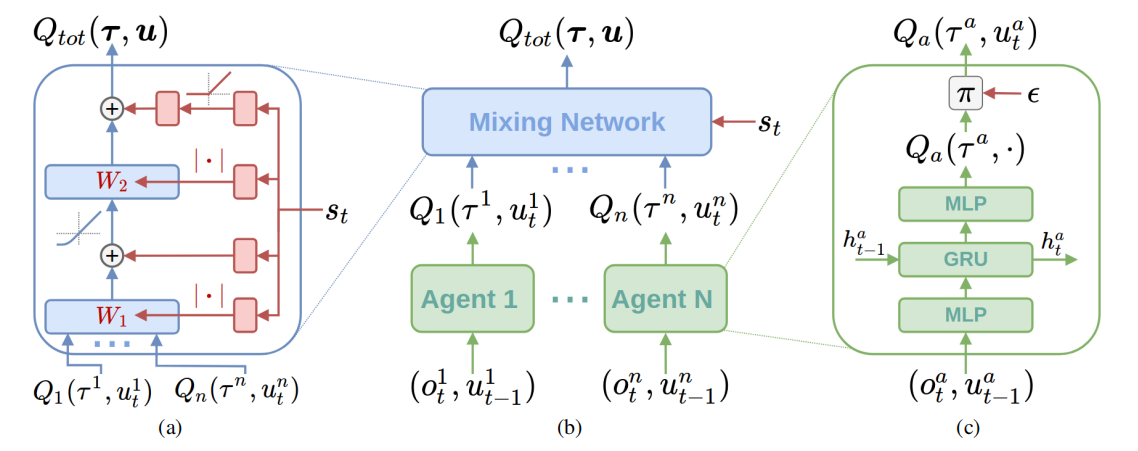
\includegraphics[width=\linewidth]{img_pfe/QMIX.PNG}
    \end{minipage}
    \hspace{0.05\textwidth} 
    \begin{minipage}{0.3\textwidth}
       
                \captionof{figure}{The QMIX architecture. (a) The mixing network ;(b) The central mixing network; (c) Agent network (Adapted from \parencite{QMIX})}
        \label{fig:qmix_architecture}
    \end{minipage}
\end{figure}
The primary advantage of this design is that the monotonicity is a sufficient condition to guarantee the \textbf{Individual-Global-Max (IGM)} principle, which ensures that a greedy action selection by each decentralized agent still corresponds to the maximization of the global team value. This allows QMIX to represent a much richer class of non-linear functions than VDN while still permitting tractable decentralized execution. However, despite its advantages, the monotonicity constraint also forms the primary limitation of QMIX, as it cannot represent non-monotonic value functions that can arise in problems where an agent's best action depends on the simultaneous actions of its teammates.

For environments with continuous action spaces, policy-gradient methods are the standard, with Multi-Agent Deep Deterministic Policy Gradient (MADDPG) being the canonical algorithm. Developed by  \parencite{MADDPG}, MADDPG adapts the single-agent DDPG actor-critic framework to the multi-agent domain by leveraging the CTDE paradigm in a unique way. While each agent's actor (policy) is decentralized and selects actions based only on its own local observations, the critic is centralized during training. Specifically, the critic is augmented with the observations and actions of all other agents. This centralized action-value function, $Q_i^{\mu}(x, a_1, \dots, a_N)$, allows the critic to form a stable learning signal, as the environment is stationary from its perspective even when other agents' policies are changing. The decentralized actor is then updated using the gradient provided by this centralized critic. The primary advantage of this structure is its flexibility and stability; it effectively solves the non-stationarity problem that challenges other methods and can be applied to cooperative, competitive, or mixed-motive settings, as each agent can learn its own unique critic and reward function. However, MADDPG's main limitation is that the input to the centralized critic grows linearly with the number of agents, which can be impractical for very large systems. Furthermore, the critic's update requires knowledge of other agents' actions during training, an assumption that, while common in simulations, can be restrictive.
% \paragraph{Multi-Agent Deep Deterministic Policy Gradient (MADDPG)}
% For environments with continuous or high-dimensional action spaces, the standard approach is the policy-gradient algorithm, Multi-Agent Deep Deterministic Policy Gradient (MADDPG). This method extends the single-agent DDPG framework by employing a specialized actor-critic architecture within the CTDE paradigm. While each agent's actor (policy) is decentralized and acts based only on its local observations, its corresponding critic is centralized during training. The critic is augmented with the observations and actions of all other agents, which provides it with a complete picture of the joint action and stabilizes the learning environment by resolving the non-stationarity problem. This allows for a robust training signal to be delivered to the decentralized actors. The flexibility of MADDPG makes it highly effective for complex control tasks, and it is often enhanced with recurrent networks and attention to better handle partial observability. Its primary limitation, however, is that policy-gradient methods are generally less sample-efficient and more computationally demanding than their value-based counterparts.
% Building upon the CTDE paradigm, this section details the influential algorithms that have defined modern cooperative MARL. These methods leverage a centralized training perspective to learn robust, coordinated policies that can be executed in a fully decentralized manner. We review the two primary algorithmic families that realize this paradigm: value-decomposition and policy-gradient methods.

% \subsubsection{Value-Decomposition Methods: Scalable Coordination}
% Value-decomposition methods are highly effective and scalable, particularly in tasks with discrete action spaces. They learn a factorized team value function ($Q_{\text{tot}}$) based on individual agent utilities ($Q_i$).

% \paragraph{VDN} As the foundational method, VDN proposes the simplest factorization, representing $Q_{\text{tot}}$ as a direct sum of individual agent values:
% $$
% Q_{\text{tot}}(\tau,u) = \sum_{i=1}^{n} Q_i(\tau_i, u_i)
% $$
% \textbf{Strength:} The primary advantage of VDN is its simplicity and scalability. \textbf{Limitation:} Its core assumption of linear additivity is a significant restriction, as it cannot represent more complex, non-linear synergies between agents.

% \paragraph{QMIX} This highly influential algorithm overcomes VDN's limitations by using a non-linear mixing network. This network takes the individual $Q_i$ values as input and combines them to estimate $Q_{\text{tot}}$. The crucial innovation in QMIX is that the mixing network's weights are constrained to be non-negative, which enforces an overall monotonicity constraint:
% $$
% \frac{\partial Q_{\text{tot}}}{\partial Q_i} \geq 0
% $$
% \textbf{Strength:} This constraint cleverly guarantees the Individual-Global-Max (IGM) principle, ensuring that a decentralized greedy selection of actions by each agent still corresponds to the optimal joint action for the team. This makes it highly effective for decentralized execution. \textbf{Limitation:} While more expressive than VDN, the monotonicity requirement still restricts the class of functions it can represent and may not capture all complex agent dependencies.

% \subsubsection{Policy-Gradient Methods: Handling Complex Actions}
% For environments with continuous or high-dimensional action spaces, policy-gradient methods are the standard. The canonical algorithm in this domain is the Multi-Agent Deep Deterministic Policy Gradient (MADDPG).

% \paragraph{MADDPG} This algorithm adapts the popular single-agent DDPG framework to the multi-agent setting using a specialized actor-critic architecture. While each agent's actor (policy) remains decentralized, acting based only on local observations, the critic is centralized during training. Specifically, each agent's critic is augmented with the observations and actions of all other agents. This global perspective allows the critic to form a stable learning target, effectively solving the non-stationarity problem.

% \paragraph{Enhancements (e.g., Zhang et al.)} The base MADDPG architecture is often enhanced to better handle partial observability. This includes integrating recurrent policies to process observation histories and adding attention mechanisms to help agents focus on the most salient information.

% \textbf{Strength:} MADDPG and its variants excel in complex, continuous action spaces and can learn sophisticated policies. \textbf{Limitation:} This flexibility comes at a cost, as these methods are generally less sample-efficient and require more computational resources and training time than their value-based counterparts.
% --------------- MAPPO----------------------------
% In the domain of policy-gradient methods, \textbf{Multi-Agent Proximal Policy Optimization (MAPPO)} \parencite{ppo_ctde} has emerged as a surprisingly effective on-policy algorithm within the CTDE paradigm. 


% MAPPO's architecture consists of a decentralized actor and a centralized critic. Each agent's actor, or policy $\pi_{\theta}(a_i|o_i)$, is decentralized, mapping its own local observation $o_i$ to an action $a_i$. The critic, or value function $V_{\phi}(s)$, is centralized and utilized only during the training phase. This centralization allows the critic to access global state information $s$ that is unavailable to the agents during execution, providing a stable learning signal that helps mitigate the non-stationarity of the multi-agent environment. For environments with homogeneous agents, the parameters for both the actor and critic networks are typically shared across all agents to improve learning efficiency.
% The policy parameters $\theta$ are optimized by maximizing the PPO clipped surrogate objective, which includes an entropy bonus term to encourage exploration. The objective function is defined as:
% \begin{equation}
% \label{eq:actor_loss}
% \mathcal{L}(\theta) = \frac{1}{Bn} \sum_{i=1}^{n} \sum_{k=1}^{B} \left[ \min\left(r_{\theta,i}^{(k)} \hat{A}_i^{(k)}, clip(r_{\theta,i}^{(k)}, 1-\epsilon, 1+\epsilon) \hat{A}_i^{(k)}\right) \right] + \frac{\sigma}{Bn} \sum_{i=1}^{n} \sum_{k=1}^{B} S[\pi_{\theta}(o_i^{(k)})]
% \end{equation}
% where:
% \begin{itemize}
%     \item $r_{\theta, i}^{(k)} = \frac{\pi_{\theta}(a_i^{(k)} | o_i^{(k)})}{\pi_{\theta_{\text{old}}}(a_i^{(k)} | o_i^{(k)})}$ is the importance sampling ratio between the current and old policies.
%     \item $\hat{A}_i^{(k)}$ is the advantage estimate calculated using Generalized Advantage Estimation (GAE).
%     \item $\epsilon$ is a hyperparameter that defines the clipping range.
%     \item $S$ is the policy entropy and $\sigma$ is its coefficient hyperparameter.
% \end{itemize}

% \noindent Concurrently, the critic's parameters $\phi$ are trained to minimize a clipped mean-squared error loss between the predicted value $V_{\phi}(s_i^{(k)})$ and the calculated reward-to-go $\hat{R}_i$. The loss is given by:
% \begin{equation}
% \label{eq:critic_loss}
% \mathcal{L}(\phi) = \frac{1}{Bn} \sum_{i=1}^{n} \sum_{k=1}^{B} \max\left[ (V_{\phi}(s_i^{(k)}) - \hat{R}_i)^2, (clip(V_{\phi}(s_i^{(k)}), V_{\phi_{\text{old}}}(s_i^{(k)}) - \epsilon, V_{\phi_{\text{old}}}(s_i^{(k)}) + \epsilon) - \hat{R}_i)^2 \right]
% \end{equation}

% The primary advantage of MAPPO is its surprising effectiveness and strong empirical performance across a variety of cooperative MARL benchmarks. The research shows that with careful tuning of key implementation factors—such as value normalization, limited training epochs, minimal mini-batching, and a small clipping ratio—MAPPO can achieve results and sample efficiency that are competitive with, or even superior to, state-of-the-art off-policy methods. Its relative simplicity and effectiveness make it an exceptionally strong baseline for cooperative MARL research. However, the analysis presented is primarily empirical, with the algorithm's performance evaluated in cooperative, discrete action spaces with mostly homogeneous agents. Its applicability to more diverse settings, such as competitive games or environments with continuous action spaces, remains a direction for future work.

As an on-policy alternative in the policy-gradient family of algorithms, \textbf{Multi-Agent Proximal Policy Optimization (MAPPO)} \parencite{ppo_ctde} offers a robust framework for cooperative multi-agent tasks. It adapts the single-agent PPO algorithm to a multi-agent actor-critic setting, leveraging the CTDE paradigm to achieve surprisingly strong performance with minimal architectural complexity.


The core of MAPPO's architecture lies in its use of decentralized actors and a centralized critic. Each agent's actor, or policy $\pi_{\theta}(a_i | o_i)$, is decentralized and maps its local observation $o_i$ to an action $a_i$. To stabilize training in the non-stationary multi-agent environment, a centralized critic, or value function $V_{\phi}(s)$, is used during the training phase. This critic has access to global state information $s$, providing a consistent and stable learning signal for all actors.


The policy parameters $\theta$ are trained by maximizing the PPO clipped surrogate objective function, which constrains the magnitude of policy updates. This objective, which also includes an entropy bonus $S$ to encourage exploration, is defined as:
\begin{equation}
\label{eq:actor_loss}
\mathcal{L}(\theta) = \frac{1}{Bn} \sum_{i=1}^{n} \sum_{k=1}^{B} \left[ \min\left(r_{\theta,i}^{(k)} \hat{A}_i^{(k)}, clip(r_{\theta,i}^{(k)}, 1-\epsilon, 1+\epsilon) \hat{A}_i^{(k)}\right) \right] + \frac{\sigma}{Bn} \sum_{i=1}^{n} \sum_{k=1}^{B} S[\pi_{\theta}(o_i^{(k)})]
\end{equation}
Where $r_{\theta,i}^{(k)}$ is the importance sampling ratio, and $\hat{A}_i^{(k)}$ is the advantage estimate calculated using Generalized Advantage Estimation (GAE).

The centralized critic's parameters $\phi$ are trained to minimize a clipped mean-squared error loss between the predicted value $V_{\phi}(s_i^{(k)})$ and the calculated reward-to-go target $\hat{R}_i$:
\begin{equation}
\label{eq:critic_loss}
\mathcal{L}(\phi) = \frac{1}{Bn} \sum_{i=1}^{n} \sum_{k=1}^{B} \max\left[ (V_{\phi}(s_i^{(k)}) - \hat{R}_i)^2, \left(clip(V_{\phi}(s_i^{(k)}), V_{\phi_{\text{old}}}(s_i^{(k)}) - \epsilon, V_{\phi_{\text{old}}}(s_i^{(k)}) + \epsilon) - \hat{R}_i\right)^2 \right]
\end{equation}
The entire system is trained on-policy, meaning that for each update, a new batch of experience is collected using the current policy. The actor and critic networks are then updated for several epochs on this data using their respective objective functions.


The primary advantage of MAPPO is its surprising effectiveness and strong empirical performance across a variety of cooperative MARL benchmarks. The research demonstrates that with specific implementation practices such as value normalization and limited training epochs, MAPPO can achieve results and sample efficiency competitive with, or even superior to, state-of-the-art off-policy methods. Its relative simplicity and generality make it an exceptionally strong baseline for cooperative MARL research. Furthermore, its performance was evaluated mainly in cooperative, discrete action spaces, with its applicability to more diverse settings remaining an open question.

\subsection{Advanced Representation Learning for Partial Observability}
While foundational algorithms like QMIX and MADDPG are powerful, they share a common approach to partial observability: each agent's observation history is typically processed by a recurrent neural network (RNN) to produce a memory or belief state. This method, however, creates a significant information bottleneck, as it compresses an arbitrarily long history into a fixed-size vector, potentially losing crucial past information. Furthermore, this implicit memory state does not allow an agent to explicitly reason about what information is missing from its view or its importance. This core limitation has motivated a shift in the research community toward more sophisticated representation learning techniques that aim to directly address the missing information, either by learning to align agent beliefs about the hidden state or by learning to reconstruct it from a partial view. In this section, we review these two approaches.


% The first advanced approach, belief alignment, is exemplified by Consensus Learning for Cooperative Multi-Agent Reinforcement Learning (COLA), introduced by \parencite{COLA}. The work is inspired by concepts from computer vision, specifically \textit{viewpoint invariance and data augmentation}, where the local observations of different agents are treated as augmented views of the same underlying global state. COLA seeks to have agents learn a shared \textbf{consensus} from these different views.

% To achieve this, COLA employs a sophisticated contrastive learning framework. While traditional contrastive learning often relies on an \textbf{InfoNCE loss} with negative sampling, COLA adopts a more recent technique inspired by \textbf{Knowledge Distillation with No Labels (DINO)}. It uses a \textbf{consensus builder} module with a student-teacher network architecture. Both networks learn to map an agent's local observation to a probability distribution over $K$ discrete classes, where $K$ is a hyperparameter representing the number of possible consensus states. The system is trained by minimizing the cross-entropy loss between the student's output for one agent's view and the teacher's output for another agent's view:
Introduced by ~\parencite{COLA}, \textbf{Consensus Learning for Cooperative Multi-Agent Reinforcement Learning (COLA)} exemplifies a belief alignment approach inspired by concepts from computer vision, specifically \textit{viewpoint invariance} and \textit{data augmentation}. The core idea is to treat the different local observations of each agent as distinct ``views'' of the same underlying global state, from which the agents learn to infer a shared consensus without communication. To achieve this, COLA employs a \textbf{consensus builder} module based on a sophisticated contrastive learning framework. Unlike traditional methods that can rely on negative sampling, COLA is inspired by \textbf{Knowledge Distillation with No Labels (DINO)}, which uses a student-teacher network architecture. This module learns to map an agent's observation to a probability distribution over $K$ discrete consensus classes. The system is trained by minimizing the cross-entropy loss between the student network's output for one agent's view and the teacher's output for another's, encouraging different views of the same state to map to the same consensus label.
% \begin{equation*}
%     L_{\text{CB}} = \sum_{a,b} H\left(P_T(z_a), P_S(z_b)\right)
% \end{equation*}

% This process trains the consensus builder to map different local observation views to the same discrete consensus label (one of the $K$ classes).
This inferred one-hot consensus is then fed as an additional input into each agent's network, providing a shared cooperative signal during decentralized execution without any communication overhead. A key strength of COLA is that it can be integrated into various CTDE algorithms like QMIX or MADDPG to improve performance with only minor changes to the model architecture. However, its effectiveness is sensitive to the hyperparameter $K$.The optimal number of consensus classes must be tuned to the task's complexity, and the approach is less beneficial in scenarios where global consensus is not required.
\begin{figure}[H]
    \centering
         
    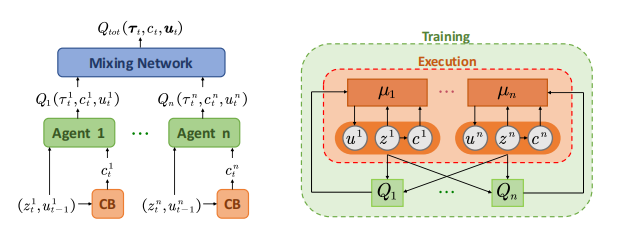
\includegraphics[width=0.6\linewidth]{img_pfe/marl_with_consensus learning.PNG}       
                \caption{Illustration of multi-agent reinforcement learning methods with consensus learning.\texttt{[Left]:} The value decomposition method with consensus learning. \texttt{[Right]:} The multi-agent actor-critic method with consensus learning (Adapted from \parencite{COLA})}
        \label{fig:marl_with_consensus_learning}
\end{figure}

% A key limitation of prior MARL representation learning methods is their primary focus on temporal awareness without explicitly learning from the rich correlational information between agents. To address this, \parencite{ma2cl} introduces the \textbf{Multi-Agent Masked Attentive Contrastive Learning (MA2CL)} framework, designed to learn representations that are simultaneously predictive in both the temporal and agent dimensions. The architecture of MA2CL, shown in Figure~\ref{fig:ma2cl_architecture}, operates as a self-supervised auxiliary task alongside a main MARL algorithm.

% The process, illustrated in Figure~\ref{fig:ma2cl_architecture}
% The process begins by "masking" a randomly selected agent by replacing its current observation and action ($o_t^i, a_t^i$) with data from the previous timestep ($o_{t-1}^i, a_{t-1}^i$). This masked sequence of observations, $\tilde{o}_t$, is passed through an Online Encoder ($\psi$) and an Online Projector ($\phi$) to produce a sequence of latent features, $\hat{z}_t$. The core of the framework is an Attentive Reconstruction model that takes this latent sequence, along with the masked actions $\tilde{a}_t$ and positional embeddings, to predict the latent representation of the masked agent, $\hat{y}_M$.




%------ MA2CL -----------------------
A key limitation of prior MARL representation learning methods is their primary focus on temporal awareness without explicitly learning from the rich correlational information between agents. To address this, \parencite{ma2cl} introduces the Multi-Agent Masked Attentive Contrastive Learning (MA2CL) framework, designed to learn representations that are simultaneously predictive in both the temporal and agent dimensions. The architecture of MA2CL, shown in Figure~\ref{fig:ma2cl_architecture}, operates as a self-supervised auxiliary task.


\begin{figure}[H] 
    \centering
    % Box for the image
        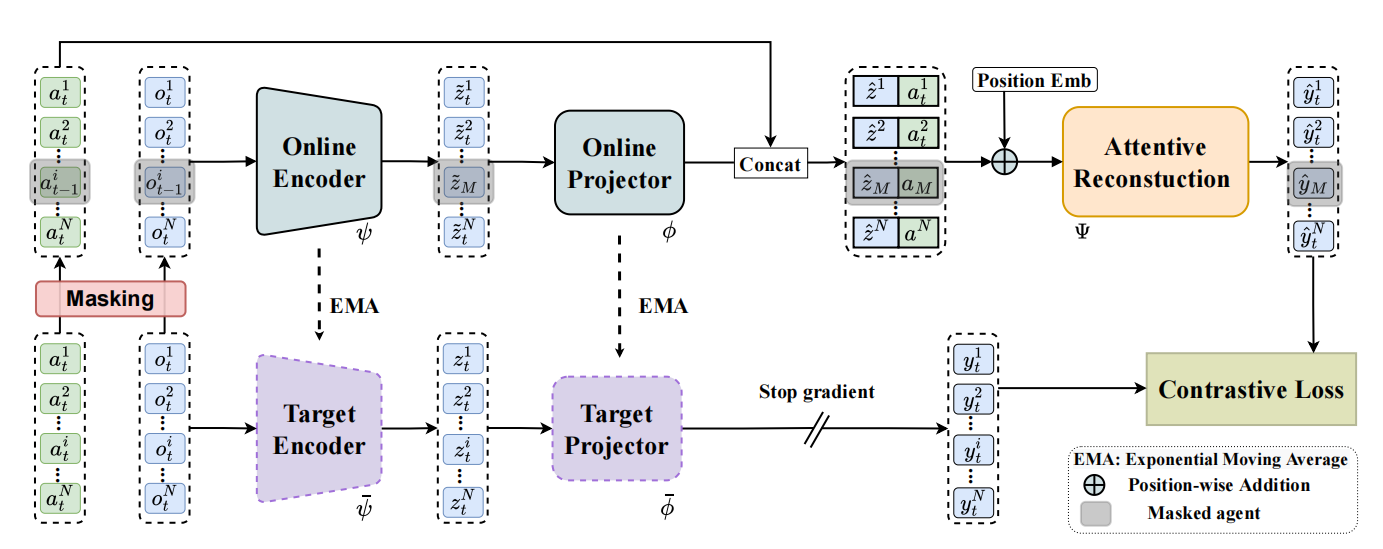
\includegraphics[width=\linewidth]{MA2CL.PNG}
   
    
        \caption{The framework of MA2CL. An online encoder and projector process masked observations, while a target network processes the original observations. An attentive reconstruction model predicts the latent features of the masked agents, which are then optimized via a contrastive loss against the target features. (Adapted from \parencite{ma2cl}).}
        \label{fig:ma2cl_architecture}
\end{figure}


It begins with a unique masking strategy in which a randomly selected agent’s current observation and action \((o^t_i, a^t_i)\) are replaced by its data from the previous timestep \((o^{t-1}_i, a^{t-1}_i)\). This masked input is then processed by a dual-stream architecture: a common design in contrastive learning, to prevent model collapse and promote stable training. An online encoder \(\psi\) and a non-linear projector \(\phi\) generate latent features from the masked data, while a target encoder \(\bar{\psi}\) and projector \(\bar{\phi}\) create stable features from the unmasked data. The target networks are updated using an exponential moving average (EMA) of the online network parameters, ensuring that target representations evolve smoothly and provide a consistent learning objective. 
An attentive reconstruction module then uses the online output to predict the masked agent’s true latent feature. The entire online network is optimized via an \textbf{InfoNCE contrastive loss} :
\begin{equation}
    \label{eq:ma2cl_loss}
    L_{\text{cl}} = \sum_{i=1}^{N} -M_i \log \left( \frac{\exp(\omega(q_i, k_i))}{\sum_{j=1}^{N} \exp(\omega(q_i, k_j))} \right)
\end{equation}

Here, the query $q_i$ is the reconstructed feature $\hat{y}_i$, the positive key $k_i$ is the true feature $y_i$ for the same agent, and the negative keys are the features $y_j$ of all other agents. This loss pushes the model to reconstruct an agent's representation accurately while distinguishing it from its teammates. 

%, which frames the prediction as a classification task: it aims to match each agent’s reconstructed latent representation to its true target representation $y_t$ among a set of distractors derived from the other agents’ features.
A \textit{stop-gradient} operation is applied to the target network outputs during loss computation to avoid a degenerate solution where both networks collapse to trivial representations. By minimizing this loss, MA2CL compels the encoder to produce rich and informative features, thereby enhancing both the quality of representation learning and the overall sample efficiency of the MARL policy.


The strength of this approach is that it forces the encoder to learn both temporal and agent-level context, significantly improving the sample efficiency and performance of the base MARL algorithm. However, a potential limitation is that such a specialized auxiliary task may encourage the representations to be highly optimized for final performance on a specific benchmark, potentially at the cost of broader generalization to different tasks.

%-------MaskMA----------------------------------
Recent work in MARL has increasingly adopted Transformer-based models to treat multi-agent decision-making as a sequence modeling problem, with notable examples including MADT\parencite{MADT}  Appendix~\ref{sec:MADT}   and MAT\parencite{MAT}  Appendix~\ref{sec:MAT}. However, these powerful architectures face two critical challenges. The first is a mismatch between their centralized training and decentralized execution; a Transformer trained on the full state of all agents struggles when executed with only partial, local observations. The second is poor generalization across tasks with varying numbers of agents and action spaces, as the meaning of the action vector can change completely from one task to another.

To address these limitations, \parencite{maskma} introduces the Mask-Based Collaborative Learning for \textbf{Multi-Agent Decision Making (MaskMA) } framework. To solve the training-execution mismatch, MaskMA employs a Mask-based Training Strategy (MTS), Figure~\ref{fig:MTS_MaskMa}. Instead of masking input tokens, it randomly masks connections within the Transformer's attention matrix during training, which forces the model to learn from partial information and thus better aligns the training phase with decentralized deployment. To handle the generalization problem, it uses a Generalizable Action Representation (GAR) that categorizes actions as either intrinsic (self-related) or interactive (other-related). By computing interactive actions based on the features of both the acting and target agents, the action representation becomes independent of the total number of agents, allowing for seamless transfer.
\begin{figure}[H]
    \begin{minipage}{0.5\textwidth}
       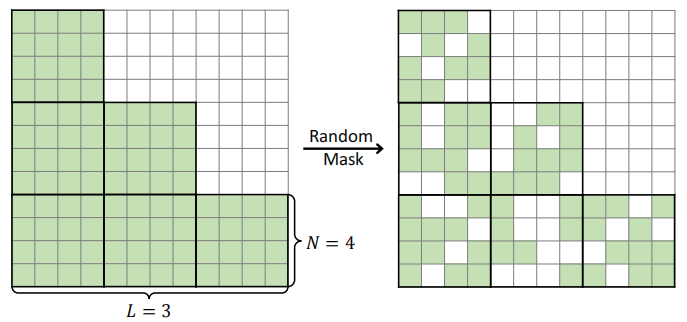
\includegraphics[width=\linewidth]{img_pfe/attention_matrix_MTS_MaskMa.PNG}
    \end{minipage}
    \hspace{0.07\textwidth} 
    \begin{minipage}{0.4\textwidth}

        \captionof{figure}{Visualization of the attention matrix in MTS. Left: The attention matrix displays a causal structure along the timestep
dimension, complemented by a non-causal configuration within each discrete timestep. Right: The final attention matrix used for training is obtained by randomly masking elements of the left attention matrix. (Adapted from \parencite{maskma}).}
        \label{fig:MTS_MaskMa}
    \end{minipage}

\end{figure}
The primary strength of this design is MaskMA's powerful zero-shot capability; the authors show that a single model trained on only 11 maps can achieve a 77.8\% win rate on 60 unseen test maps and can adapt to dynamic downstream tasks like ad hoc team play and ally malfunction. However, the framework's main limitation is its reliance on pre-collected, high-quality expert datasets for its imitation learning approach, and its generalization to entirely new game environments beyond its training domain is an area for future work.

% While prior self-supervised methods like MA2CL and MaskMA introduced masking to MARL, they often neglect the natural structure of partial observability, where an agent's local view is inherently a masked version of the global state. To address this, \parencite{ma2rl} proposes Masked Autoencoders for Multi-Agent Reinforcement Learning (MA2RL), a framework that improves agent collaboration by explicitly modeling and reconstructing the relationship between observed and unobserved entities. The MA2RL process first uses a Variational Autoencoder (VAE) to encode all observable entities into a latent space. Then, a recurrent network (GRU) uses this latent information and historical context to infer the representations of all unobserved (masked) entities. This reconstructed global view of all entities is then used to select a task-independent skill. Finally, an attentive action decoder generates an action based on both the skill and the complete (observed + inferred) entity information. A key aspect of this approach is the joint training of the reconstruction module and the policy itself, allowing the representation learning to be directly guided by the policy's needs. \textbf{The primary strength of MA2RL} is that by explicitly reasoning about and reconstructing the unobserved world from an entity perspective, it learns more generalizable and useful representations for coordination, leading to strong zero-shot performance. \textbf{However, this complex architecture}, which involves joint optimization of multiple components including VAEs and a policy network, may require more training steps and careful handling of multiple supervision signals to converge effectively.

%-----------MA2RL---------

While prior skill-based methods struggle to achieve team awareness under partial observability, and other masking techniques like MA2CL use \textit{artificial} masking strategies, a more direct approach is needed to handle an agent's limited view. These earlier methods do not treat an agent's line of sight as a natural mask of the full environment from an entity-centric perspective. To address this specific problem, \parencite{ma2rl} proposes Masked Autoencoders for Multi-Agent Reinforcement Learning (MA2RL). The core idea of MA2RL is to treat partial observability as a natural masking problem from an \textbf{entity perspective}. It views the environment as a collection of entities (allies, enemies, etc.), where an agent's local observation is simply a partial list of these entities, and all others are considered \textbf{masked} by being out of sight.

The MA2RL framework Figure~\ref{fig:ma2rl_architecture} and Figure~\ref{fig:ma2rl_att_decoder}  is designed to reconstruct a complete picture of the environment by inferring the states of these unobserved entities. It first uses a Variational Autoencoder (VAE)\parencite{vae} to encode the visible entities into a latent space. Then, a recurrent network (GRU) uses this information and past history to infer the latent representations of all the currently unobserved (masked) entities. This reconstructed global view, containing both observed and inferred entities, is then used to learn more generalizable, task-independent skills. The primary strength of this approach is its ability to learn a rich and complete representation of the world, leading to improved coordination and remarkable zero-shot generalization capabilities. However, the framework's complex, multi-component architecture, which jointly optimizes VAEs, a recurrent network, and the policy, may require significant training steps and careful management of its various supervision signals.

\begin{figure}[H] 
    \centering
    % Box for the image
        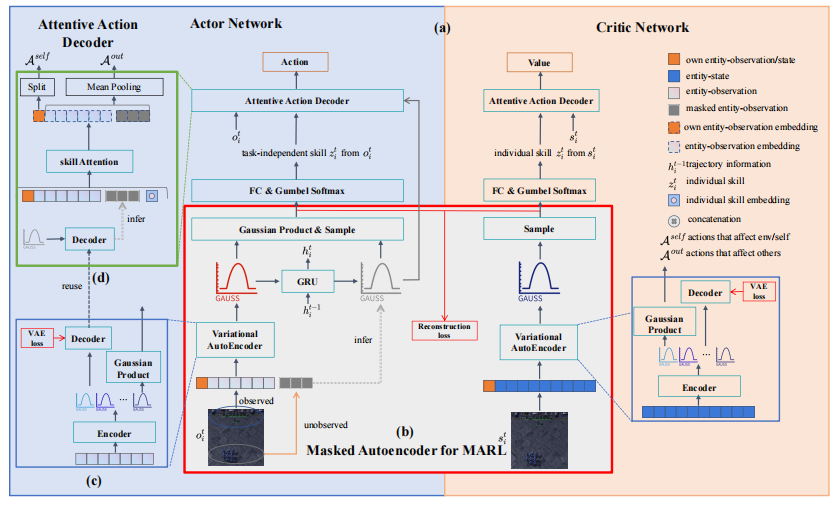
\includegraphics[width=\linewidth]{img_pfe/MA2RL.PNG}
   
    
        \caption{The network structure of MA2RL. (a) The overall architecture. (b) The structure of VAE. (c) The details of the masked autoencoder for MARL, where entity-observations can be regarded as a mask of the entity-states. (d) The attentive Action decoder that reuses the decoder in
VAE to infer masked entity-observations for better action execution. (Adapted from \parencite{ma2rl}).}
        \label{fig:ma2rl_architecture}
\end{figure}

\begin{figure}[H] 
    \centering
    % Box for the image
        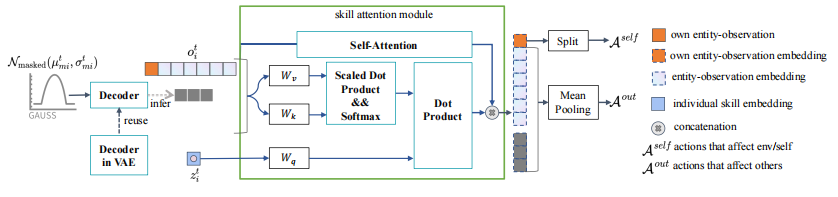
\includegraphics[width=\linewidth]{img_pfe/MA2RL_att_decoder.PNG}
   
    
        \caption{Attentive action decoder. The attentive action decoder utilizes the latent representations of all masked entity-observations to infer the information of masked entities and then applies a skill attention module to obtain the action. (Adapted from \parencite{ma2rl}).}
        \label{fig:ma2rl_att_decoder}
\end{figure}


%---------- MA2E ---------
% While approaches like communication are not always feasible and abstract consensus methods can be lossy, other representation learning techniques like MA2CL or MaskMA are often tightly coupled with the policy network or designed for different objectives like action prediction. To address the need for a more general and modular information inference module,  \parencite{ma2e} proposes the Multi-Agent Masked Auto-Encoder (MA2E). The core idea of MA2E is to use a masked autoencoder to explicitly reconstruct the full trajectories of all agents, conditioned only on the partial trajectory of a single agent. This is achieved by taking the trajectories of all agents, applying agent-level masking (i.e., completely masking out the information of several random agents), and training a Transformer-based autoencoder to reconstruct the original, complete data by minimizing the Mean Squared Error.

% A key differentiator of MA2E is its decoupled, two-stage training process. First, the MA2E module is pre-trained using data from a random policy until it can reliably reconstruct the global information. Then, during the main MARL training, the policy network is trained according to its own objective, while the pre-trained MA2E module is periodically fine-tuned. During decentralized execution, each agent feeds its own local trajectory into its MA2E module to infer a reconstructed global view, which is then used to augment its decision-making. 
% The primary strength of this decoupled design is its modularity and transferability; MA2E can be easily plugged into various existing value-based or policy-based MARL algorithms to significantly boost their performance and sample efficiency. However, the framework has two main limitations: its inference capability degrades when agents are too far apart for their observations to overlap, and its architecture is not designed to easily scale to environments with a varying number of agents.
While approaches like communication are not always feasible and abstract consensus methods can be lossy, other representation learning techniques like MA2CL or MaskMA are often tightly coupled with the policy network or designed for different objectives like action prediction. To address the need for a more general and modular information inference module,
\parencite{ma2e} proposes the Multi-Agent Masked Auto-Encoder (${MA}^2E$). The core idea is to use a masked auto-encoder, built on a Transformer architecture, as a plug-in module for existing CTDE algorithms. During training, the module learns to reconstruct the full trajectories of all agents after having the trajectories of a random subset of agents masked out. This self-supervised task forces the agent to learn a rich latent representation that implicitly contains inferred global information. This representation is then used by the agent's policy for more effective decentralized decision-making. 
The primary strength of ${MA}^2E$ is its ability to significantly improve the sample efficiency and final performance of strong baselines like QMIX, achieving results comparable to having full state information. However, the framework's effectiveness is limited in scenarios where agent observations do not overlap, as there is no information from which to infer the state of distant agents. Furthermore, its architecture is not inherently designed to scale to a dynamically varying number of agents.



%---------- MACKRL ---------

While the CTDE paradigm addresses the non-stationarity of the learning problem, a fundamental limitation persists in many of its implementations, such as COMA \parencite{COMA} or QMIX \parencite{QMIX}. In these frameworks, the requirement for fully decentralized policies during execution often forces agents to ignore potentially useful local information, as acting on it could make their behavior unpredictable to teammates and hinder coordination. To address this, \parencite{mackrl} proposes an alternative paradigm that explicitly leverages common knowledge: information that a group of agents all possess, and all know that they all possess it.


\begin{figure}[h!]
    \begin{minipage}{0.55\textwidth}
       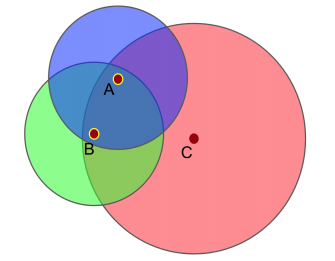
\includegraphics[width=\linewidth]{img_pfe/agent_fov.png}
    \end{minipage}
    \hfill
    \begin{minipage}{0.4\textwidth}

        \captionof{figure}{Three agents and their fields of view (for more details, Annexe~\ref{sec:mackrl_details}). A and B’s locations are common knowledge to A and B as they are within each other’s fields of view. Although C can see A and B, it shares no common knowledge with them. (Adapted from \parencite{mackrl}).}
        \label{fig:agents_fov}
    \end{minipage}

\end{figure}

% \begin{wrapfigure}{r}{0.45\textwidth} % 'r' means float to the right, '0.45\textwidth' is the width
%     \centering
%     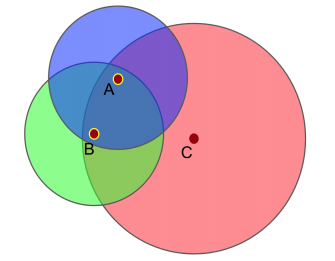
\includegraphics[width=0.4\textwidth]{img_pfe/agent_fov.png}
%     \caption{Three agents and their fields of view (for more details, Annexe~\ref{sec:mackrl_details}). A and B’s locations are common knowledge to A and B as they are within each other’s fields of view. Although C can see A and B, it shares no common knowledge with them. (Adapted from \parencite{mackrl}).}
%     \label{fig:agents_fov}
% \end{wrapfigure}
% \begin{figure}[H]
%     \centering

%     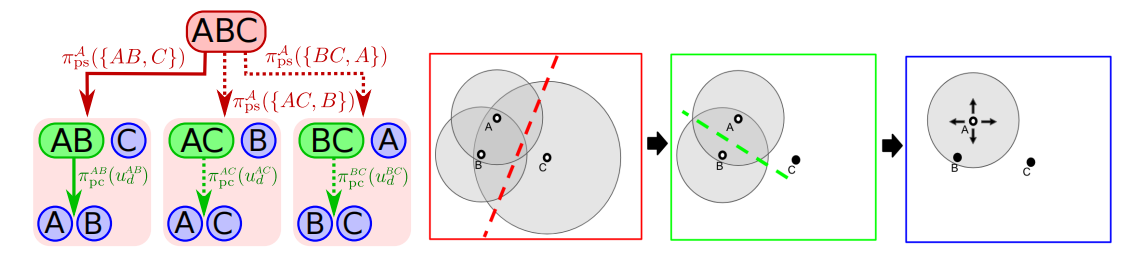
\includegraphics[width=\linewidth]{img_pfe/MACKRL_arch.PNG}
%     % \caption{The hierarchical policy tree of Pairwise MACKRL for three agents. The top-level pair selector chooses a partition (e.g., \{AB, C\}). The pair controller for AB then decides whether to take a joint action or delegate control to the individual agent policies. (Adapted from \parencite{mackrl}).}
%     \caption{
%         An illustration of Pairwise MACKRL.(Adapted from \parencite{mackrl})
%         \texttt{[left]:} the full hierarchy for three agents (dependencies on common knowledge are omitted for clarity). Only solid arrows are computed during decentralised training, while all arrows must be computed recursively during centralised training. 
%         \texttt{[right]:} the (maximally) 3 steps of decentralised sampling from the perspective of agent A.
%         \begin{enumerate}
%             \item Pair selector $\pi_{\text{ps}}^{ABC}$ chooses the partition $\{A,B,C\}$ based on the common knowledge of all agents $\mathcal{I}^{ABC}(\tau^A, \xi) = \emptyset$.
%             \item Based on the common knowledge of pair A and B, $\pi_{\text{pc}}^{AB}(\tau^A, \xi)$, the pair controller $\pi_{\text{pc}}^{AB}$ can either choose a joint action $(u_{\text{env}}^A, u_{\text{env}}^B)$, or delegate to individual controllers by selecting $u_d^{AB}$.
%             \item If delegating, the individual controller $\pi^A$ must select the action $u_{\text{env}}^A$ for the single agent A. All steps can be computed based on A's history $\tau^A$.
%         \end{enumerate}
%     }
%     \label{fig:mackrl_arch}
% \end{figure}

\begin{figure}[H]
    \centering
    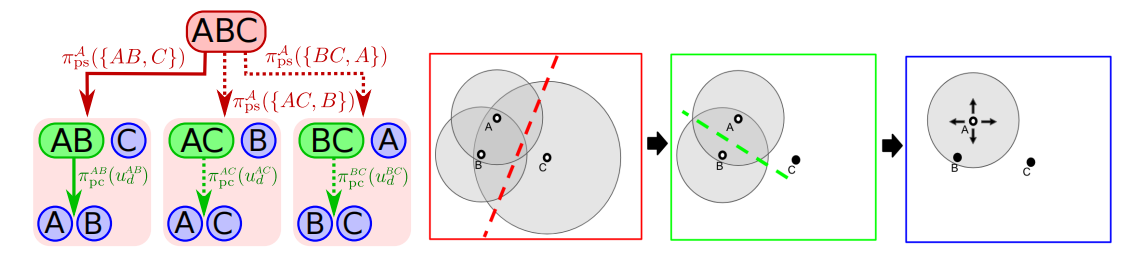
\includegraphics[width=\linewidth]{img_pfe/MACKRL_arch.PNG}
    
    % --- The Caption ---
    % The main caption text goes here.
    \caption{An illustration of Pairwise MACKRL. 
    \texttt{[left]:} the full hierarchy for three agents (dependencies on common knowledge are omitted for clarity). Only solid arrows are computed during decentralised sampling, while all arrows must be computed recursively during centralised training. 
    \texttt{[right]:} the (maximally) 3 steps of decentralised sampling from the perspective of agent A. 
    (Adapted from \parencite{mackrl})}
    \label{fig:mackrl_arch}

    \begin{minipage}{\linewidth}
    \begin{enumerate}
        \item Pair selector $\pi_{\text{ps}}^{ABC}$ chooses the partition $\{A,B,C\}$ based on the common knowledge of all agents $\mathcal{I}^{ABC}(\tau^A, \xi) = \emptyset$.
        \item Based on the common knowledge of pair A and B, $\pi_{\text{pc}}^{AB}(\tau^A, \xi)$, the pair controller $\pi_{\text{pc}}^{AB}$ can either choose a joint action $(u_{\text{env}}^A, u_{\text{env}}^B)$, or delegate to individual controllers by selecting $u_d^{AB}$.
        \item If delegating, the individual controller $\pi^A$ must select the action $u_{\text{env}}^A$ for the single agent A. All steps can be computed based on A's history $\tau^A$.
    \end{enumerate}
    \end{minipage}

\end{figure}

The core idea of Multi-Agent Common Knowledge Reinforcement Learning (MACKRL) is that when common knowledge (for more details, see Annexe~\ref{sec:mackrl_details}) is available, when agents are within each other's line of sight, they can execute complex, coordinated joint actions without the need for communication. The architecture operationalizes this through a hierarchical policy tree, as illustrated in Figure~\ref{fig:mackrl_arch}. Higher levels in this hierarchy learn to coordinate groups of agents by conditioning their joint actions only on their shared common knowledge. If sufficient common knowledge is not available or if coordination is not required, these higher-level controllers can delegate control to lower levels in the tree, which correspond to smaller subgroups or even individual, fully decentralized policies. The entire policy tree is learned end-to-end using a centralized critic, but because all decisions are based on information that each agent can independently deduce (its own local history plus what is common knowledge), the policy can be executed in a fully decentralized manner.

The primary strength of MACKRL is its ability to learn a flexible policy that dynamically switches between tight, joint-action coordination and independent decision-making, based on the information available at any given moment. This allows it to outperform both purely decentralized methods (like IQL) \parencite{Independent_vs_Cooperative_Agents} and other centralized training approaches in specific coordination-heavy benchmarks. However, the framework's main limitations are its scalability and its reliance on a pre-defined common knowledge function. The number of possible agent partitions for the top-level controller grows factorially with the number of agents, making it difficult to scale. Furthermore, the method requires a function to identify when and what common knowledge exists, which may not be available or easy to define in all environments.


% \section{Literature Review}
% \subsection{From Independent to cooperative agents}
% Multi-agent systems can be used to address problems in a variety of domains, including robotics, distributed control, telecommunications, and economics. The complexity of many tasks arising in these domains makes them difficult to solve with pre-programmed agent behaviors. The agents must instead discover a solution on their own, using learning. One of the first papers that addressed the integration of independent agents in a multi-agent system was \cite{IQL}. The author proposed independent policies for each of the agents. The learned decision policy was to be determined by the state-action value function: 
% \begin{equation}
%     Q(x,a) \leftarrow Q(x,a) + \alpha (r+\gamma V(y) - Q(x,a)) 
% \end{equation}
% Using Boltzmann distribution: 
% \begin{equation}
%     p(x,a_i) = \frac{e^{Q(x,a_i)/T}}{\sum _k e^{Q(x,a_k)/T}}
% \end{equation}
% This allows working with a continuous action space, and by adjusting the temperature, we can vary the degree of randomness in action selection. High temperatures lead to more exploratory behavior, while lower temperatures prioritize exploitation. However, IQL still faced many limitations, amongst which are the Partial Observability of the Environment, because when dealing with centralized learning, the agents are only guided by a partially observable environment whose dynamics are in constant change, and the Non-Stationarity of the Environment, due to the fact that independent Algorithms face non-stationarity in Multi-Agent domains due to the violation of the Markovian property in a Markov Decision Process. Thus, convergence is not always guaranteed. 

% In 2017, Foerster et al. introduced a new framework for cooperative agents, "Counterfactual Multi-Agent Policy Gradients" \cite{COMA}. COMA uses a centralized critic (that conditions on true global state $s$ or the joint action-observation histories) to estimate the Q-function and decentralized actors (these are agents receiving feedback from the critic to update their policies) to optimize the agents’ policies. In addition to addressing the challenges of multi-agent credit assignment, it uses a counterfactual baseline that marginalizes a single agent’s action while keeping the other agents’ actions fixed. Agents are in a fully cooperative Multi-agent task $G=\langle \ S, \ U, \ P, \ r, \ Z, \ O, \ n, \gamma \  \rangle$, each of them has a history of action-observation history $\tau ^ a$. Their joint policy induces a state-value function:
% \begin{equation}
%     V^{\pi } (s_t) = E[R_t/s_t]
% \end{equation}
% and an action-state function:
% \begin{equation}
%     Q^{\pi } (s_t, u_t) = E[R_t/s_t, u_t]
% \end{equation}
% The critic's feedback is represented mathematically by an advantage function, comparing the Q-values for current $u^{a}$ to a counterfactual baseline (inspired by reward difference):
% % \begin{equation}
% %     A (s, u) = Q(s, u) - \sum _{u'^{a}} \pi ^{a} (u' ^{a} / \tau ^{a} )  Q(s, (u^{-a} , u' ^{a} )) 
% % \end{equation}

% When dealing with the limitations of IQL (partial observability and non-stationarity), the authors of COMA estimate the advantage of an agent's action by comparing the value of the joint action to counterfactual scenarios where the agent took different actions. All other agents' actions are fixed while computing the advantage function.  A schematic of COMA model during training is shown in Figure C.3 in Appendix C.

% These two papers represented two extremes in the study of cooperation in multi-agent systems and served as an inspiration to many papers aiming to find a middle ground between independent agents and agents working collectively in a centralized setting. Amongst these were:
% \begin{itemize}
%     \item \cite{VDN} which addresses the challenges of cooperative MASs with a single joint reward signal by training individual agents using a novel architecture that decomposes the team value function into agent-wise value functions.
%     \item \cite{QMIX}, which is a value-based method that enables training decentralized policies in a centralized manner by estimating joint action values through a complex non-linear combination of per-agent values based solely on local observations.
%     \item \cite{QTRAN} which introduces a factorization method for multi-agent reinforcement learning tasks in centralized training with a decentralized execution regime.
%     \item \cite{LOLA} which allows each agent to shape the anticipated learning (policies specifically) of the other agents in the environment. This resulted in passive-aggressive behavior from agents. 
% \end{itemize}

% And \cite{PED}, whose authors proposed a value-based deep MARL method that gradually reshapes the rewards in a distributed manner such that the agent’s perception of the equilibrium gears toward optimizing social welfare. The PED-DQN framework can be used in semi-cooperative tasks through decentralized learning with induced peer evaluation. The key challenge in semi-cooperative tasks is selfishness, which is represented by separate reward functions, which often result in the agents choosing non-cooperative actions. 

% Achieving maximum cooperation was quantified by obtaining the optimal policy: 
% \begin{equation}
% \begin{split}
%     \pi ^{*} = & \ (\pi ^{*}(u_1, o_1),  \pi ^{*}(u_2, o_2), ....., \pi ^{*}(u_n, o_n)) \\ 
%      \pi ^{*} = & \ \text{argmax} _{\pi} \sum _a  E[r_a(s,u)]
% \end{split}
% \end{equation}
% The reward update requires that agents' actions become socially optimal ones that maximize cooperation and that they all have access to feedback from peers.

% They proposed reshaping the reward function using a peer evaluation metric, quantified by: 
% \begin{equation}
%     z_a ^t = r_a ^t + \gamma max _u Q_a ^M (o_a ^t , u | \theta ^{M'} _a ) - Q_a ^M (o_a ^t , u_a ^t | \theta ^{M'} _a )
% \end{equation}
% The reshaped reward is: 
% \begin{equation}
% \begin{aligned}
%         \hat{r}_a = & r_a + f_1
%         \\ \hat{r}_a = & r_a +\beta Z_a
%     \\ Z_a = & \frac{1}{|K_a|} \sum _k z_k ^t
% \end{aligned}
% \end{equation}
% The PED-DQN paper uses two neural networks:
% \begin{enumerate}
%     \item \textbf{AQDN: }used to select an action with the maximum Q-value for a given observation, where the target is:
%     \begin{equation}
%         y_a ^A (o'_a, r_a | \theta _a ^{A'}) = r + \gamma max Q^{A} (o'a, u'_a | \theta _a ^{A'}
%     \end{equation}

    
%     \item \textbf{MQDN: } used to calculate the peer evaluation signal, where the target is:
%     \begin{equation}
%         y_a ^M (o'_a, r_a | \theta _a ^{M'}) = \hat{r} + \gamma max Q^{M} (o'_a, u'_a | \theta _a ^{M'})
%     \end{equation}
% \end{enumerate}
% A faster learning rate is used for the MDQN, which updates for quasi-stationary ADQN. The PED-DQN framework, despite giving good results in semi-cooperative settings, still lacked a distributed Peer Evaluation system, assuming agents can be forced to be prosocial and did not weigh on the reputation or the trust of agents. The mechanism of the PED-DQN paper and the Distribution of the peer evaluation scores between agents and their neighbors are shown in Figures C.1 and C.2 in Appendix C.



% In 2019, Zegers et al. introduced in \cite{FCLT} a new mechanism to account for agents' reputations. The idea behind the paper was to develop distributed event-triggered controllers for heterogeneous agents, allowing them to achieve formation control and leader tracking, with resilience to adversarial Byzantine agents. A reputation-based approach is used for the agents to discern between cooperative and Byzantine neighbors, and then selectively disregard Byzantine state information. We will give further insights into this paper in section 2.3.4.


% \subsection{Reward Engineering}
% Reward Engineering is a critical aspect of designing intelligent agents, particularly in complex and dynamic environments. It involves shaping the reward functions that guide the learning process of agents, ensuring that they receive appropriate feedback for their actions. Effective reward engineering can significantly influence the efficiency and effectiveness of learning algorithms, enabling agents to achieve desired outcomes more reliably. By incorporating both extrinsic rewards (based on external goals and tasks) and intrinsic rewards (based on the agent's internal motivations and curiosity), we can create a more efficient and flexible learning framework. 

% Agents in a MAS may be cooperative, competitive, or may exhibit some mixture of these behaviors. Based on the state space, action space, and the goals of the learning, we can either add a reward shaping mechanism or a reward reshaping mechanism. \textbf{Reward Shaping} involves adding additional rewards to the original reward function to guide the agent toward desired behaviors. The primary goal is to make learning more efficient by providing intermediate rewards that help the agent understand which actions are beneficial in the long term. \textbf{Reward Reshaping} refers to modifying the reward function based on the agent's ongoing experience to better reflect the desired outcomes. This approach adjusts the reward signals dynamically as the agent interacts with the environment. The reward function is not static and can be altered during training based on the agent's performance and emerging patterns. Reward Shaping is typically designed and fixed before training begins, while Reward Reshaping occurs during the training process, allowing for dynamic updates to the reward function.

% In both these scenarios, the reshaping function that is added to the base reward function can be modeled through 2 methods: 


% \subsubsection{PBRS (Potential Based Reward Shaping):} 

% This is defined as: 
%     \begin{equation}
%         F(s,s')=\gamma \phi (s') - \phi (s) 
%     \end{equation}
    
%     where $\phi (s)$ is the potential function that returns the potential for state s, and γ is the same discount factor used when updating value function estimates. PBRS has been proven not to
% Alter the optimal policy of a single agent acting in infinite-horizon and finite-horizon MDPs.

% The form of PBRS described above can, however, only represent domain knowledge as a preference for different states, and does not provide any information to the agent regarding spe-
% Specific actions that may be beneficial. PBRS was extended to allow the knowledge
% regarding favorable actions to be included. This extension is called Potential-Based Advice. As
% part of this extension, the potential function is expressed for a state-action pair. This was proposed under two different forms of Potential-Based Advice: 


% \textbf{Look-Ahead Advice:}
% \begin{equation}
%     F(s,a,s',a') = \gamma \phi (s',a') - \phi (s,a)
% \end{equation}

% \textbf{Look-Back Advice:}

% \begin{equation}
%     F(s,a,s',a') =  \phi (s',a') - \gamma ^{-1} \phi (s,a)
% \end{equation}


% In order to guarantee policy invariance for Look-Ahead Advice in single-agent learning scenarios, certain additional criteria must be satisfied. Specifically, how an agent selects actions must be modified so that its policy $\pi$ chooses the action that will maximize the sum of Q-value and potential. However, for the Look-Back Advice, no corresponding proof of policy invariance for a single agent
% learning with Look-Back Advice has been published, although empirical results suggest that Look-Back Advice does not modify the optimal policy in single-agent learning scenarios. 


% \subsubsection{Difference Rewards:} This form of reward shaping is only applicable to cooperative MAS; therefore, only stochastic fully cooperative multi-agent domains are considered in this work. Different rewards are inspired by the intuition that all
% agents in a cooperative MAS should try to contribute to the global utility, and make use of a
% global utility function G.


% A difference reward $D_i$ is a shaped reward signal that aims to quantify each agent’s individual contribution to the system performance in a cooperative MAS:
% \begin{equation}
%     D_s (s_i, a_i) = G(s,a) - G(s_{-i} \cup s_i ^{c} , a_{-i} \cup a_i ^{c})
% \end{equation}

% where $G(s, a)$ is the global system utility, s is the system state, a is the joint action, and $(G(s_{-i} \cup s_i ^{c}, a_{-i} \cup a_i ^{c})$ is the counterfactual which represents the global utility for a theoretical system without the contribution of agent $i$.
% The terms $s_{-i}$ and $a_{-i}$ refer to all the states and actions not involving agent $i$, while $s_i ^{c}$ and $a_i ^{c}$ are fixed states and actions not dependent on agent $i$. Typically, the counterfactual system utility is calculated with agent $i$ removed, or by assuming a default state/action for agent $i$.

% \subsection{Intrinsic Reward}
% Intrinsic rewards, derived from the agent's own experience and introspection, can significantly enhance learning in environments where agents partially cooperate but also pursue individual goals. In such semi-cooperative settings, the introspective reward mechanism allows agents to evaluate and adjust their strategies based on past successes and failures, leading to more adaptive and resilient behavior. This approach fosters a balance between individual learning and collective success, ensuring that agents remain effective and aligned with the overarching objectives of the environment.

% In the next paragraphs, we shed light on multiple works highlighting the use of intrinsic rewards in cooperative, competitive, or coordination games. These studies demonstrate how intrinsic rewards can drive innovation in agent strategies, and enhance cooperation among agents.

% \subsubsection{Cooperation and Reputation Dynamics with RL}


% The goal of this intrinsic reward is achieving stabilizing cooperation in a MAS using a reputation-based approach, by combining two mechanisms: seeding a proportion of the system with fixed agents that steer others towards desired equilibria and introducing intrinsic rewards based on the idea of introspection, inspired from evolutionary game theory (EGT will be defined in the next chapter). It is based on social norms; which are functions that translate how the actions of the parties involved in an interaction, translate into their future reputation (whether agents are seen as good or bad), for example:
% \begin{enumerate}
%     \item \textbf{$0000_2$}: Actions and reputations play no role. 
%     \item \textbf{$0011_2$}: Cooperating with others is always "good" and defecting is always "bad".
%     \item \textbf{$1001_2$}: An agent that cooperates with others with good reputation and defects to those whose reputation is bad is a good agent.
%     \item \textbf{$1011_2$}: Someone is "bad" only if they refuse to cooperate with a good individual.
% \end{enumerate}
% We reshape the reward such as "Agents care about what their policy would do to an agent like themselves."
% \\ The reward becomes:
%     \begin{equation}
%             R_i = \alpha U_i + (1- \alpha) S_i
%     \end{equation}
% with: $U_i$ the payoff in a particular encounter, $S_i$ the payoff they would get if they faced themselves, and $\alpha$ is the level of introspection.

% \subsubsection{Gifting}

% Instead of opponent modeling (like the LOLA model, or using SST (state space vectors) to model the other agents in the environment), gifting allows agents to influence each other's actions, decisions, and strategies without taking the risk of having passive-aggressive behavior during the learning. Gifting extends
% the action space of learning agents in coordination games to allow rewards to be
% transferred among agents. To increase the probability of reaching the prosocial equilibrium in settings with multiple equilibria, This work investigates adding zero-sum gifting actions, so that agents may decide to give some of their rewards to others, preserving the
% total reward of agents.

% For each player, a new set of actions is defined: 

% \begin{equation}
%     \sigma_i : G_1 \ \text{x} \ G_2 \ \text{x} \  \cdots \ \text{x} \  G_N \rightarrow \mathbb{R}
% \end{equation}

% where: 
% \begin{equation}
% \begin{aligned}
%     \forall & g_i \in G_i: g_i \geq 0, 
%     \\ \sigma _i & (g) = -g_i + \frac{1}{N-1} \sum _{j \in -i} g_j
%     \end{aligned}
% \end{equation}
% $g_i$ is the gifting action of agent $i$, $g_j$ the gifting action of its peers $j \in -i$, $g$ denotes the gifting action of all agents, and $\sigma _i$ formulates how the payoff of agent $i$ changes with the gifting actions it receives from its neighbors. The corresponding payoff function for each agent is then: 
% \begin{equation}
%     \Bar{\mu} _i (\Bar{s}) = \mu _i (s) + \sigma _i (g) 
% \end{equation}
% where $\Bar{\mu} _i$ is the payoff function for agent $i$, $\Bar{s} = (s,g)$, $\mu _i (s)$ is the reward the agent $i$ got from executing its own action following its own policy, and $\sigma _i (g)$ accounts for the additional reward or gifts that were sent out by other agents.


% Since $\sum _{i=1} ^N \sigma _i (g) = 0 $, introducing the gifting actions into
% the game does not change the total reward among all agents.

% Figure C.4 in Appendix C shows the technique used in the paper of Seeding agents to promote cooperation. Panel A shows the average cooperation in the last half of the episodes. Panel B shows typical learning trajectories for the population of agents using an efficient social norm. Panel C shows the results for norm 0 $0000_2$: where actions and reputations play no role.

% \subsubsection{Contrastive Introspection:}

% In order to address the issue of long-term credit assignment and the sparse rewards problem, the authors present an approach using offline contrastive learning, which they call Contrastive Introspection. While the agent is training, ConSpec stores the observations’ knowledge in a collection of prototypes summarizing the intermediate states required for success. When an agent arrives at any state that matches one of these prototypes, it gets an additional intrinsic reward to the already established external rewards. This reshaped reward is only taken into consideration if the similarity score exceeds 60$\%$, and if it is the maximum of 6 scores taken in a time window of 6 $(t-3, \cdots,  t, \cdots, t+3)$:
% \begin{equation}
%     \Tilde{r}_{kt} = \lambda \sum ^H _ {i=1} \hat{s}_{ikt} \cdot 1_{\hat{s}_{ikt} = max \{ \hat{s}_{ik, t-3}, \cdots , \hat{s_{ik, t+3}} \} }
% \end{equation}

% ConSpec (as seen in the figure C.5 in the Annex) uses three memory buffers: one for the current mini-batch being trained (B, with a capacity of MB), one for successful episodes (S, with a capacity of MS), and one for failed episodes (F, with a capacity of MF). Each episode consists of T time steps. Our findings indicate that these memory buffers don't need to be very large for ConSpec to function effectively; 16 slots in memory suffice, even for 3D environments. Each buffer stores the raw observations, Ot, encountered by the agent. When a new mini-batch of observations is loaded into B for training, episodes are categorized into successes and failures based on the criteria described in A.1. Observations from these categorized episodes are then stored in S and F in a first-in-first-out (FIFO) manner, with older episodes being overwritten as new ones arrive.




% \subsubsection{Learning from Demonstration}
% This reward relies on the principle of Demonstrator or Expert, which can be used in Reinforcement Learning to encourage faster learning of the agents by giving them access to the state-action pairs that had good quality values. Reward shaping based on this principle can be very beneficial if the reshaping function is well-engineered: 
% \begin{equation}
%     R_F (s,a,s') = R(s,a,s') + F(s,a,s')
% \end{equation}
% The potential function defined for the reward shaping chosen in this work is: 
% \begin{equation}
%     F(s,a,s') = \gamma \phi (s') - Q(s)
% \end{equation}
% This definition was extended by others to include actions and time-steps, allowing for the incorporation of behavioural knowledge that reflects the quality of actions as well
% as states, and allowing the shaping to change over time:
% \begin{equation}
%     F(s,a,t,s',a',t') = \gamma \phi(s',a',t') - \phi (s,a,t)
% \end{equation}
% As in Reinforcement Learning, an agent operating in a Learning-from-demonstration setting looks for a policy π that allows it to execute a certain task. While
% in RL, the agent has a reward signal to evaluate its behavior, this evaluation metric is not present in the Learning from Demonstration setting (similarly for inverse reinforcement learning), and the agent
% must refer to expert demonstrations (sequences of state-action pairs
% {(s0, a0 ), . . . , (sn, an )}) of the task to derive a policy that mimics and generalizes these demonstrations.

% Here, the reshaping function is defined as a Gaussian similarity measure over the state
% space:
% % \begin{equation}
% %     g(s,s^{d} , \sum ) = e^{- \frac{1}{2} (s-s^{d}^{T} \sum ^{-1} (s-s^{d}))}
% % \end{equation}
% By incorporating this expression in the potential function $\phi$, we get:
% % \begin{equation}
% %     \phi (s,a) = max _{s^{d} , a ) g(s,s^{d} , \sum )
% % \end{equation}
% The way the agent collects the experiences is as follows: once the agent's learning starts, at the end of each episode, the Q-value $\hat{q}(s_t , a_t)$ for each state-action in this episode is Monte Carlo estimated until the final time step T :
% \begin{equation}
%     \hat{q}(s_t , a_t) = \sum ^{T} _{k=t} \gamma ^{k-t} r_t
% \end{equation}
% The state-action pairs and their estimated Q values are then stored in a priority queue with the estimated Q-values being the sort key of the queue. If the queue is full (defined by queue size parameter qs), only state-action pairs with a higher estimated Q- value than the smallest in the queue are added (and the smallest are consequently removed). The agent looks into the priority queue (that represents now a queue for the demonstrator experiences) and calculates the potential function:
% \begin{equation}
%     \phi (s,a) = \phi max _{(s^{d} , a)} g(s,s^{d} , \sum ) \hat{q}(s_t , a_t) 
% \end{equation}
% where $\phi$ is a hyper parameter the authors of this paper defined as a scaling factor to control the exploration of the agent.

% \subsubsection{Introspective Learning through queries:} 
% This introspective reward aims to carry out counterfactual reasoning over unrealized events. The authors of the paper introduced an introspection oracle to query the agent on whether there exist states in which the agent would select certain actions. The algorithm uses this data to train and to improve the
% safety of the agent without requiring that such potentially dangerous
% situations be encountered in real life. We shed light on what highlights this reward:
% \begin{itemize}
%     \item Working on a pre-MDP $(D=(S,A,p))$ consisting of a set of states S, set of actions A, and transition probabilities $p(s, a, s′)$.
%     \item $\pi (D)$ is the set of all policies for D. Opt(M) is the subset of $\pi (D)$ containing optimal policies for M. M being the set of all MDPs over D.
%     \item Working with terminal pairs $(S,A)$ instead of terminal states.
%     \item $Pr(X)$ is the set of all well-behaved subsets of $X \in R_n $. Well-behaved subsets $S \times A$ are the ones defined with non-linear function symbols (for example: speed/acceleration).
% \end{itemize}
% We define an introspective oracle for policy $\pi$ as a map:
% \begin{equation}
%     w_{\pi} : Pr (S \times A) \rightarrow \{ \bot \} + S
% \end{equation}
% with $\bot$ indicates an error, or in other terms, the pair was not found in time. If $w_{\pi} (U)=s$ then the pair is found, where $U$ refers to the property of the pair (state, action). We query the state
% $s = w(U_i)$, and if it is found, then $(w_{\pi} (U), \pi(w_{\pi} (U))$ is in $U$. The examples gathered are inserted into the replay buffer as terminal.


% These introspective rewards can all be helpful for the agents for faster learning and faster convergence. However, in the scenario of the gifting model, agents can become greedy and selfish with passive-aggressive behavior. The cooperation and reputation dynamics paper introduced social norms to the environment, which can limit its dynamics (in an Atari game, prey-predator..). The introspective learning through queries takes into consideration the future mistakes that an agent can make and helps them avoid them by making those states terminal and ending the episode. Finally, the contrastive reward took into account the state-action pairs with the highest values as prototypes for the agents to learn from. Although both these methods, in addition to the learning from demonstration method, have led to good results in simulations, they were not very efficient in a semi-cooperative prey-predator scenario. 


% \subsection{Byzantine agents}

% We start by defining the \textbf{Byzantine Generals' Problem}: A number of generals are attacking a fortress. The generals must decide as a group and agree on a common decision: whether to attack or retreat 
% $\rightarrow$ If only a few generals attack, it is worse than a coordinated attack or a coordinated retreat. 

% There are two types of Byzantine agents, and each one has a type of attack that compromises the decision-making process:
% \begin{enumerate}
%     \item \textbf{Byzantine Agents type I: } remains in the mobile network, where it can delay or corrupt information communicated to its neighbors (Feeding false information like the generals who vote to attack but will retreat).
%     \item \textbf{Byzantine Agents type II: } Abandons the mobile network while communicating true or no state information about itself (like generals who will eventually attack but maybe with different allies). 
% \end{enumerate}


% \begin{figure}[hbt!]
%   \centering
%   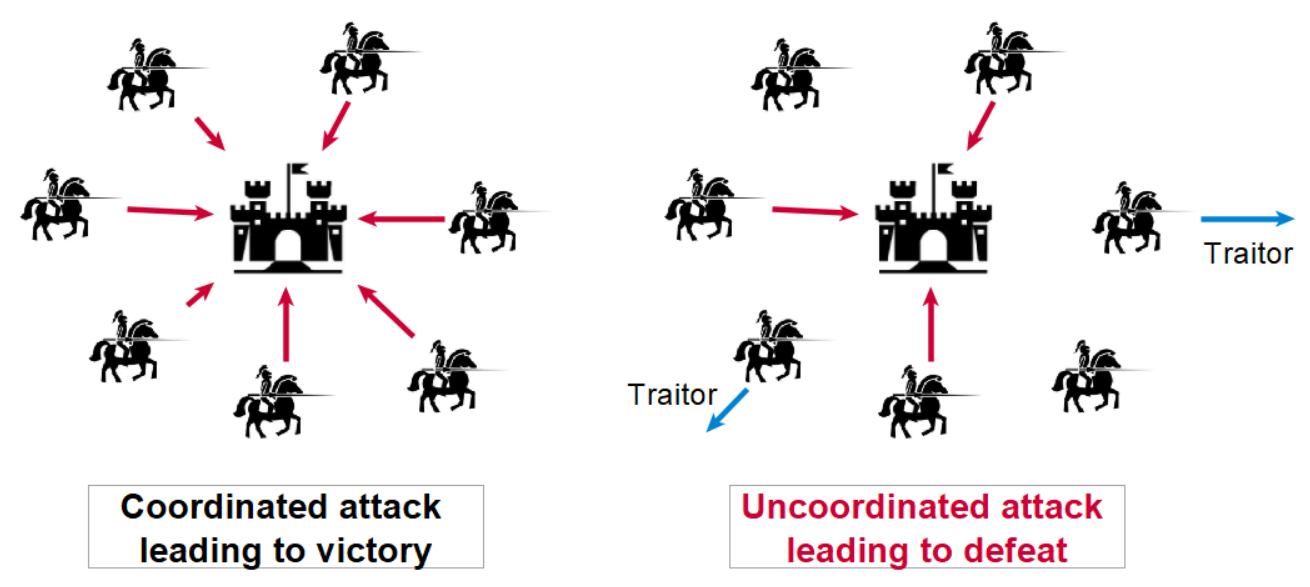
\includegraphics[width=0.8\textwidth]{images_pfe/1_xJGKNqJVrkFVtZ6NggwHbw.png}
%   \caption{A representation of the Byzantine agents.}
% \end{figure}
% \FloatBarrier

% As we already stated in the previous section, the inspiration behind this work is to develop distributed event-triggered controllers for heterogeneous agents, allowing them to achieve formation control and leader tracking, with resilience to adversarial Byzantine agents. A reputation-based approach is used for the agents to discern between cooperative and Byzantine neighbors, and then selectively disregard Byzantine state information. We define:
% \begin{itemize}
%     \item $B: [0, \infty [ \rightarrow 2 ^ \nu$ : time-varying set of Byzantine agents.
%     \item $C: [0, \infty [ \rightarrow 2 ^ \nu$ : time-varying set of Cooperative agents.
% \end{itemize}
% This leads to $ B(t) \cap C(t) = \emptyset $ and $B(t) \cup C(t) = \nu $ (the leader not included).
% \vspace*{0.1cm}
% The agent's dynamics were modeled as an uncertain non-linear model for the agent's velocity: 
% \begin{equation}
%     \dot{x}_i(t) = f_i (x_i(t)) + g_i (x_i(t)) u_i(t) + d_i(t), \forall \ i  \in  \mathlarger{\nu} \cup  \{ 0 \}
% \end{equation}
% Where: 
% \begin{itemize}
% \item \textbf{$f_i$:} $R^n \rightarrow R^n$: \textbf{uncertain drift dynamics}: describe the long-term behavior or trend in an agent's motion that can be influenced by uncertain disturbances.
%     \item \textbf{$g_i$:} $R^n \rightarrow R^{n*m}$: \textbf{known control effectiveness matrix}: describes how the control inputs for each agent affect the entire system's state. 
%     \item \textbf{$u_i$:} $[0, \infty ) \rightarrow R^m$: \textbf{control input}.
%     \item \textbf{$d_i$:} $[0, \infty ) \rightarrow R^n$: \textbf{exogenous disturbance} for agent i: the external influence that affects the behavior/dynamics/state of the agent. 
% \end{itemize}
% As for the controllers' development, the authors proposed a model based on 4 steps: 
% \begin{enumerate}
%     \item Building a trust model
%     \item Building a reputation model
%     \item Study of an edge weight policy
%     \item Building an event-triggered control mechanism for each agent
% \end{enumerate}
% However, this mechanism faces certain limitations; the need for a ground truth, the need for an accurate state estimation of all agents, and the lack of distinction between Byzantine agents and Cooperative agents in the absence of the ground truth.


\section*{Conclusion}
This review of the state-of-the-art has traced the evolution of cooperative MARL algorithms, from foundational value-decomposition networks like VDN and QMIX to more advanced representation learning frameworks designed to overcome partial observability. While methods like COLA and MACKRL introduce clever ways to share or align agent information, they can be limited by abstract representations or restrictive assumptions. More recent approaches based on masked auto-encoding, particularly ${MA}^2E$, have shown great promise by learning to reconstruct a global view from local observations. However, as identified in our analysis, ${MA}^2E$'s reliance on a policy-agnostic, random masking strategy represents a key limitation, creating a disconnect between the representation learning task and the agent's actual learning progress. It is this specific gap that necessitates a masking strategy dynamically informed by the MARL training process itself, which motivates the novel contribution presented in the next chapter.


